%Introduction
In this chapter I present a brief introduction of the
LHC physics, the CMS detector, and the physics behind the off-shell methods
for constraining Higgs decay width. Finally, a very brief technical account for
the Monte Carlo (MC) events production.

\section{Physics at LHC}
After the discovery of Standard Model (SM) Higgs boson in 2012, the Large Hadron Collider (LHC)
went through a series of upgrades during Long Shutdown 1 (2013-2015) and finally restarted with center-of-mass energy reaching
\SI{13}{\tera\electronvolt}. Though the last particle promised by the SM has been discovered,
no Supersymmetry (SUSY) particle has been spotted so far.

The null results has not discouraged physicists from other attempts of probing the 
beyond the Standard Model (BSM) physics in other ways. Higgs boson has a special role in
the process mainly due to the Higgs field which it originates from couples to massive particles
and could be a window to probe BSM the physics, as discussed in Section \ref{sec:physics_offshell}.

The LHC has been operating at the same energy for the past 3 years (2016-2018) and each year
the delivered luminosity as been ramping up.\cite{xampl} In this analysis, we will be using
simulation that corresponds to Run period 2018, which in turn corresponds to a 
\SI{59.74}{\per\femto\barn} luminosity for the Compact Muon Solenoid (CMS) detector.\cite{xampl}

\section{The CMS Detector}
% [1]CMS Collaboration. Performance of CMS muon reconstruction in pp collision events at sqrt(s) = 7 TeV. J Inst 2012;7:P10002–P10002. https://doi.org/10.1088/1748-0221/7/10/P10002.

% [2]CMS Collaboration. Performance of electron reconstruction and selection with the CMS detector in proton-proton collisions at sqrt(s) = 8 TeV. J Inst 2015;10:P06005–P06005. https://doi.org/10.1088/1748-0221/10/06/P06005.

% [3]Cacciari M, Salam GP, Soyez G. FastJet user manual. Eur Phys J C 2012;72:1896. https://doi.org/10.1140/epjc/s10052-012-1896-2.

% [4][0802.1189] The anti-k\_t jet clustering algorithm n.d. https://arxiv.org/abs/0802.1189 (accessed May 25, 2020).
The CMS is one of the two general purpose detectors built around LHC (the other one is ATLAS). It
is `compact' only when comparing to the ATLAS detector and is in fact heavier than the latter.
Though we are not using the data accumulated by the CMS detector, the simulated events are
reconstructed based on the material and electronics responses of the real detector using the
\gf package.\cite{geant4}

The defining feature of the CMS detector is the solenoid (as in its name) around the beam line.
This superconducting solenoid produces a \SI{4}{\tesla} magnetic field and is 
\SI{12.5}{\meter} long free bore.\cite{validation_cms} This feature allows the track of
any charged particle (given the momentum is not ridiculously high) to be bent when penetrating
the detector layers and leave behind a track which provides information regarding the particle's 
electric charge.


\begin{figure}[htb]
\begin{center}
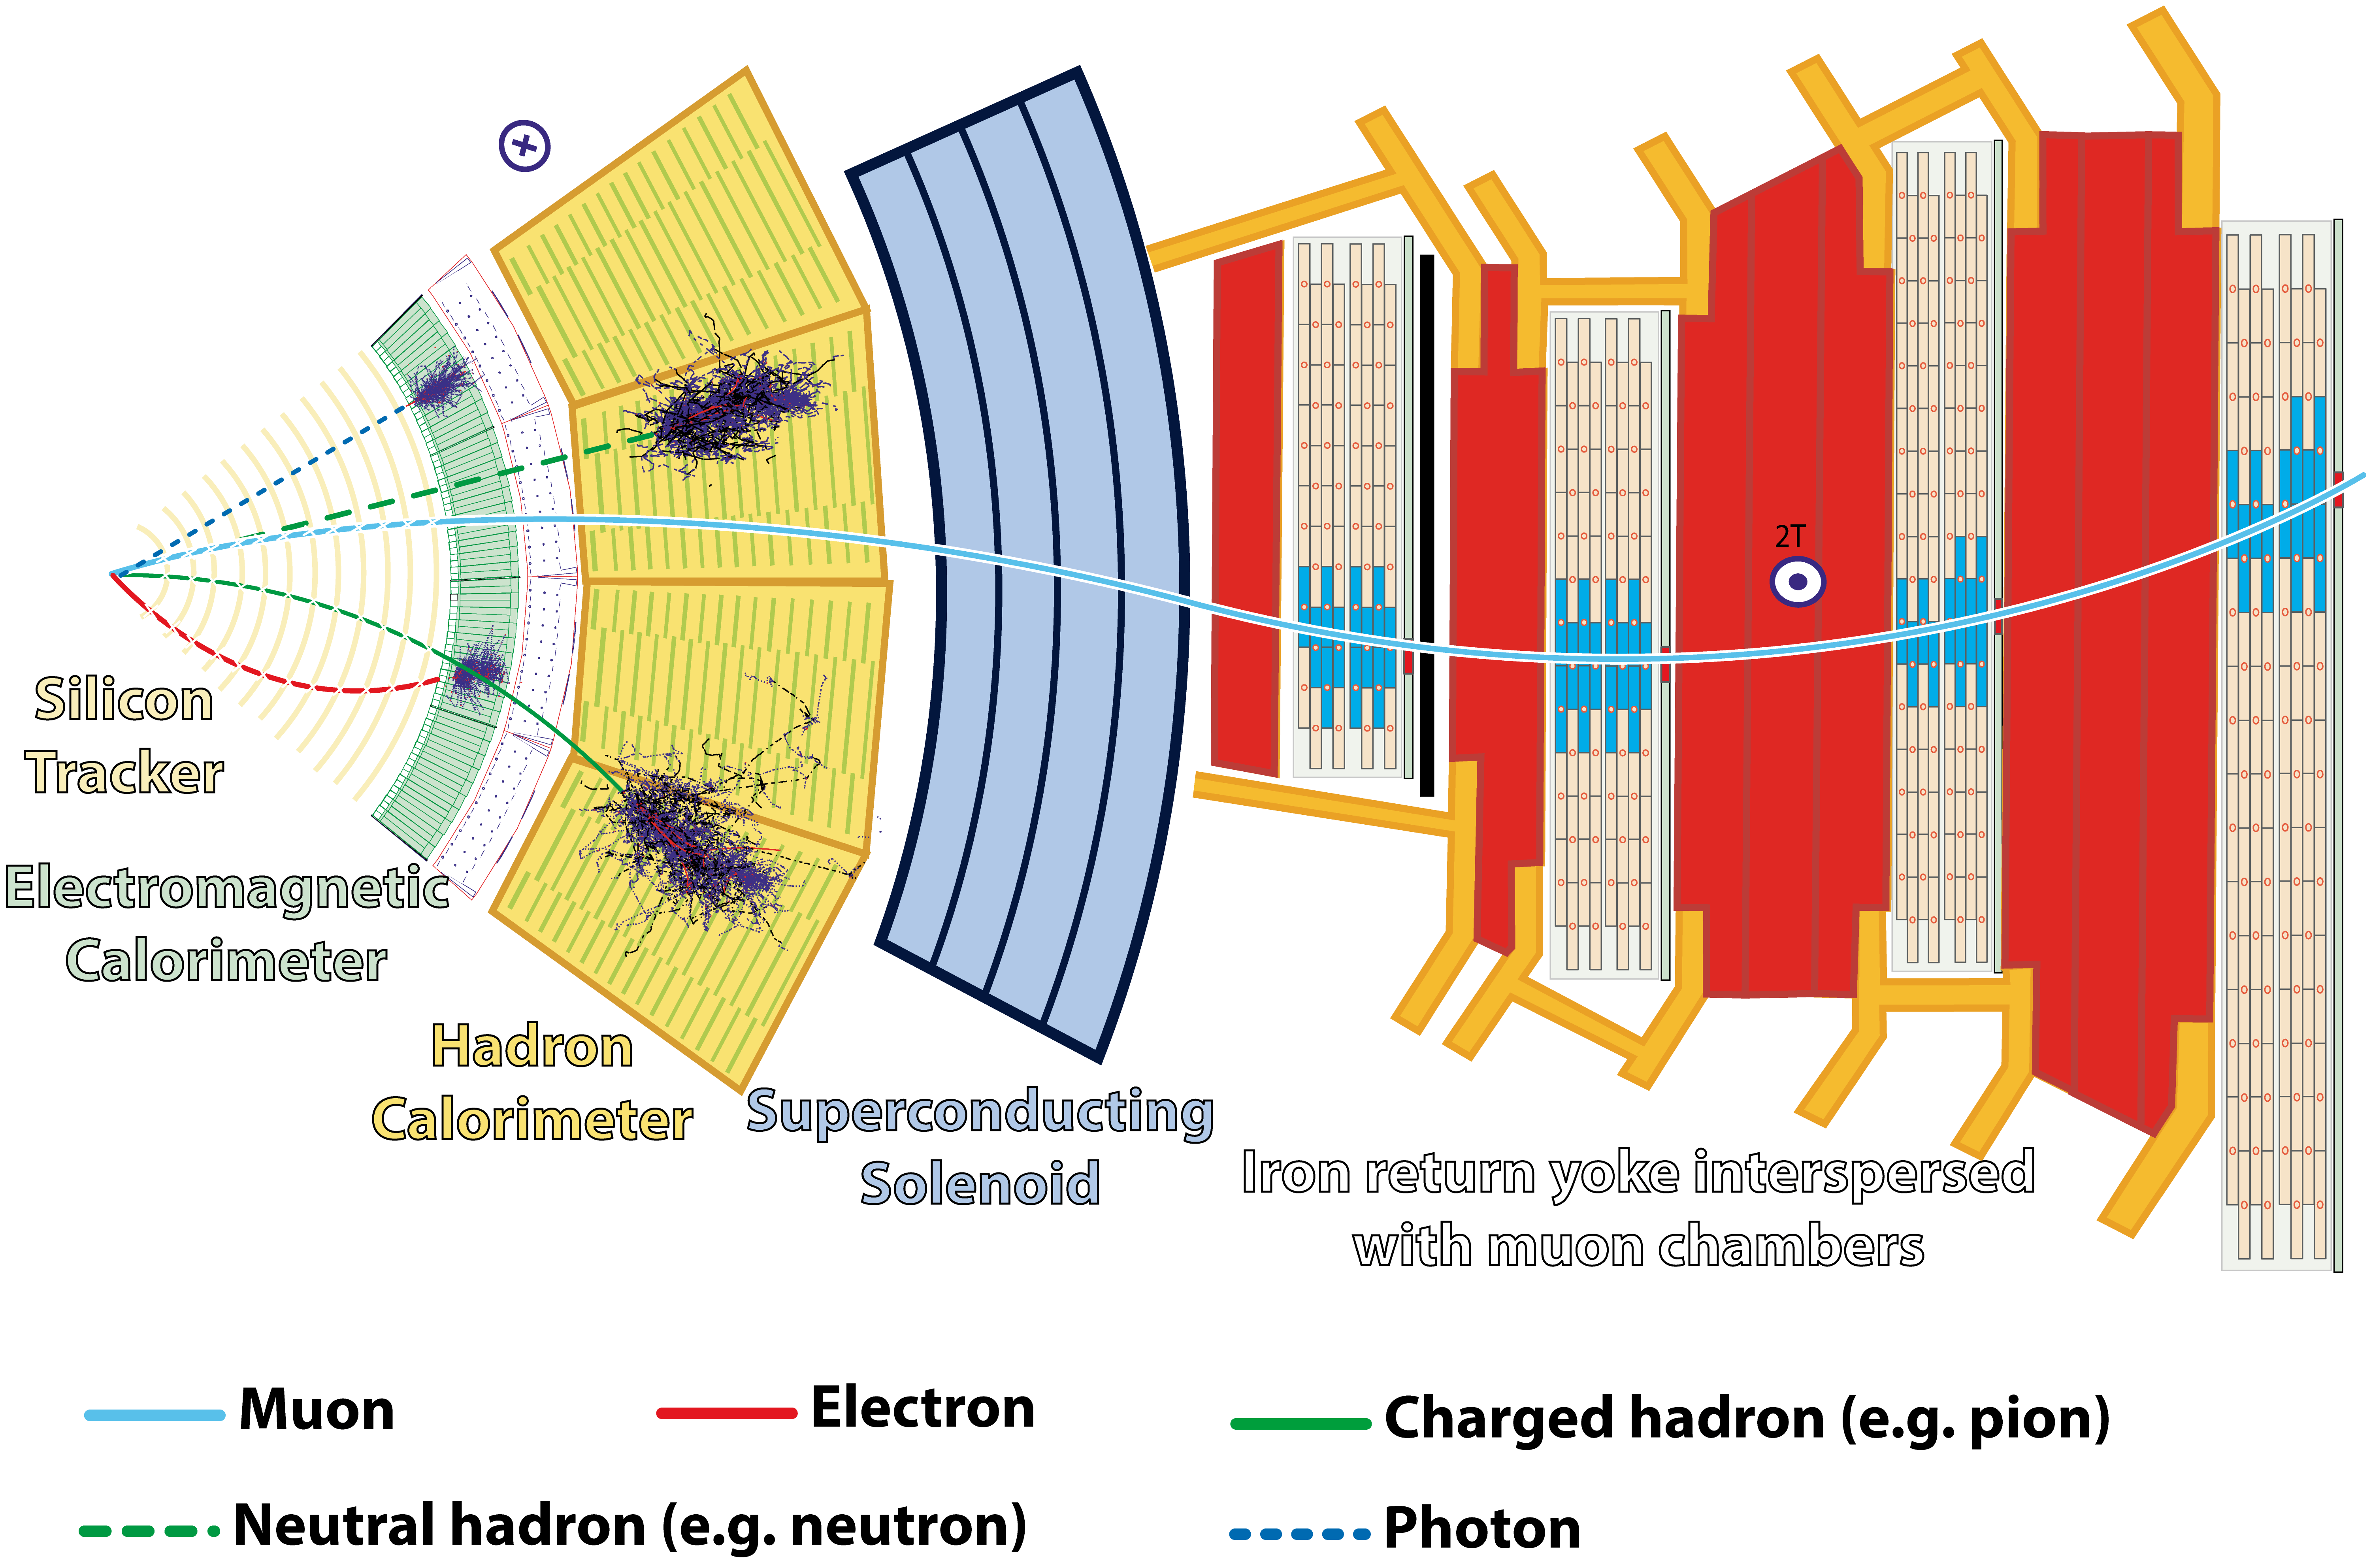
\includegraphics[width=.75\linewidth]{fig/CMS_Slice.png}
\end{center}
\caption{A section slice of the CMS detector where we can see how 
particles with different physical properties interact differently with the detector.}
\label{fig:CMS_Slice}
\end{figure}

One important kind `final-state' particles used in this thesis this charged lepton, 
which includes electrons and muons (half-life of tauon is too short);
`final-state' here means they are the end products of decay chain and interact with detector
components directly. If we concentrate on the red and blue lines in \ref{fig:CMS_Slice}, we
can see that for the electrons (red), they leave a few hits (4) that resemble a curved
track within the Silicon Tracker layer and are stopped at the Electromagnetic Calorimeter
(ECAL). 

For the muons (blue line in \ref{fig:CMS_Slice}), they largely go through all the interior layers unhinged due to their
high mass; pay close attention to the `S'-shaped curve, this is due to the opposite magnetic
field outside of the superconducting solenoid. Although information such as momentum relies on
hits on the silicon tracker, the hits in the muon chambers and a matching trajectory is needed 
for the object to be reconstructed as a muon. Notice how the
muon chambers occupy more than half of the detector by size, such design allows the CMS 
detector to excel in muon measurements and is the primary reason for the overall design.
% \todo[inline]{TODO: PF and anti-k algorithm in the context of this thesis}

Zooming out from the individual component of the CMS detector, the complete reconstruction
process is complex and sometimes requires information from multiple parts of the detector, this
algorithm is called the Particle Flow (PF) \cite{particle_flow}. While simple and neutral object like photon whose 
energy is directly measure by the ECAL (with correction for zero-suppression), electron measurements
need the information from the inner tracker (one way to determine momentum), energy at the ECAL, and
also sum of the energy of photons produced by bremsstrahlung compatible with the electron's track.

For gluons and quarks that come out of the interaction vertex, due to quark confinement, the detector 
is only be able to `see' a narrow `spray' of final state (stable) particles whose collection is called `jet'.
There are different ways and criteria to combine a collection of measurements into a single physical object,
and in CMS, the anti-$k_t$ clustering algorithm is used. In short, the algorithm would cluster objects
in a cone (meaning it has a fixed $\eta-\phi$ space) originated from the vertex according to some parameter.
But it also needs to be resilient to QCD effects that would cause jet to split, such as shown in Fig.
\ref{fig:jet_split}, where previous generation of algorithm may misidentify them.

\begin{figure}[htb]
\begin{center}
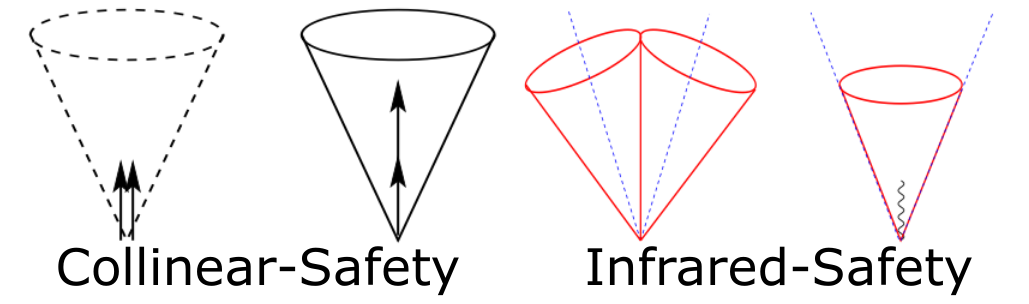
\includegraphics[width=.85\linewidth]{fig/jet_split.png}
\end{center}
\caption{A illustration of two kinds of QCD effects in jets\protect\footnotemark}
\label{fig:jet_split}
\end{figure}
\footnotetext{\url{https://twiki.cern.ch/twiki/bin/viewfile/Sandbox/Lecture?rev=1;filename=Philipp\_Schieferdeckers\_Lecture.pdf\#page=3}}

In this analysis, we use the AK4 jets which means that the algorithm is given a $R=0.4$ parameter, another
common choice is $R=0.8$ which is preferred in some cases for boosted topologies due to a larger `opening
angle'.

\section{The Higgs boson and off-shell methods}\label{sec:physics_offshell}
[1]Caola F, Melnikov K. Constraining the Higgs boson width with ZZ production at the LHC. Phys Rev D 2013;88:054024. https://doi.org/10.1103/PhysRevD.88.054024.

The importance of a Beyond the Standard Model (BSM) physics is self-evident, though the SM is one
of the most precise theory in physics we ever had, the model requires many `inputs' from experiment
for parametrization, and, it cannot account for phenomena such as neutrino oscillation with its
original form. While the direct searches in the past few years have all yield null results,
many indirect probing have been going as well.

As mentioned above, the Higgs boson has a special place as it can be seen as a `bridge' between
the SM and the BSM (in some models) as some SUSY particles can decay into it or it can decay
into SUSY particles, or simply have a BSM production Feynman diagram that leads to more Higgs
bosons than the SM would expect. In any of these cases, the basic properties of the SM Higgs
boson remain important.

Many properties are well measured, such as it's mass and spin \cite{higgs_papers}, others, however,
have not entered the realm of `precision' physics so far. One of them is the decay width of
the Higgs boson, which is of course associated to the particle's half-life. The SM predicts
that the Higgs boson to have a decay width of \SI{4.1}{\mega\electronvolt}. The problem is
that the energy resolution of the CMS detector, which is around $\mathcal{O}(1)$\si{\giga\electronvolt}
for the di-photon or 4-leptons final states, is not even remotely small enough to check this 
prediction directly.

I will give a very brief account\cite{ulascan} for the proposed (and been completed in previous years' run)
method that can constrain the Higgs decay width using events that fall into the off-shell
tail.

When the Higgs boson decays to two vector bosons (VV), in the scope of this thesis, two Z bosons,
either one of the vector bosons is off-shell, or the Higgs boson is off-shell, this is because
$m_\text{H}\approx\SI{125}{\giga\electronvolt}$ is smaller than the 
mass of two \PW{}'s($\approx\SI{160}{\giga\electronvolt}$) 
or two \PZ{}'s($\approx\SI{182}{\giga\electronvolt}$). The Higgs boson decay branching ratio
is coupled to the daughter particles' mass thus this cross section
$\sigma_{\mathrm{H}\rightarrow\mathrm{VV}}$ is enhanced as the mass of Higgs boson gets closer to 
the on-shell VV mass.  

In fact, the production of Higgs boson from a pair of vector boson is also related to the
decay width of Higgs boson $\Gamma_\text{\PH}$ via the propagator term. In terms of the
differential cross section:
\be
\label{eqn:diff_xsec}
\frac{\mathrm{d} \sigma_{\mathrm{vv} \rightarrow \mathrm{H} \rightarrow \mathrm{VV}}}{\mathrm{d} q_{\mathrm{H}}^{2}} 
\sim 
\frac{g_{\mathrm{vvH}}^{2} g_{\mathrm{HVV}}^{2}}{\left(q_{\mathrm{H}}^{2}-m_{\mathrm{H}}^{2}\right)^{2}+m_{\mathrm{H}}^{2} \Gamma_{\mathrm{H}}^{2}}
\ee
where the two $g$ on the right-hand side are the couplings for production from VV and decay
to VV respectively. Integrating this equation near the on-shell mass of the SM Higgs boson 
or in the tail region (above the mass of VV), one can translate the differential cross section
into event rate that can be (in theory) measured in experiments:
\begin{equation}
\begin{split}
&N_{\mathrm{vv} \rightarrow \mathrm{H} \rightarrow \mathrm{VV}^{*}}^{\text{on-shell}} \sim \frac{g_{\mathrm{vvH}}^{2} g_{\mathrm{HVV}}^{2}}{m_{\mathrm{H}} \Gamma_{\mathrm{H}}} \sim \mu_{\mathrm{vvH}}
\\
&N_{\mathrm{vv} \rightarrow \mathrm{H}^{*} \rightarrow \mathrm{VV}}^{\text{off-shell}} \sim \frac{g_{\mathrm{vvH}}^{2} g_{\mathrm{HVV}}^{2}}{\left(2 m_{\mathrm{V}}\right)^{2}} \sim \mu_{\mathrm{vvH}} \cdot \Gamma_{\mathrm{H}}
\end{split}
\end{equation}
The key takeaway is that, up to some correction factors, the event rates of off-shell scales
linearly respect to the Higgs decay width $\Gamma_\text{\PH}$ which allows us to indirectly
measure the width itself.

In this thesis, we will focus on the $\mathrm{H} \rightarrow \mathrm{ZZ} \rightarrow 2\ell2\nu$ channel
at the CMS detector using simulated (MC) events. This work done here is part of the ongoing work
within a group formed by UCSB HEP group, Universit\'e Libre de Bruxelles, and Beihang University under
the CMS Collaboration\footnote{Internally, CMS AN-20-081}. The analysis items and methods included in this
thesis is a subset of what will be in the official analysis and is a part of the final measurement. More
detail on what approximation has been taken in order to obtain a preliminary expected result is discussed
in the next few sections.

% \todo[inline]{maybe elaborate a bit more?}
% \newpage\phantom{blabla}


\section{Background and signal simulation}
% [1]Agostinelli S, Allison J, Amako K, Apostolakis J, Araujo H, Arce P, et al. Geant4—a simulation toolkit. Nuclear Instruments and Methods in Physics Research Section A: Accelerators, Spectrometers, Detectors and Associated Equipment 2003;506:250–303. https://doi.org/10.1016/S0168-9002(03)01368-8.

% [2]Gritsan AV, Roskes J, Sarica U, Schulze M, Xiao M, Zhou Y. New features in the JHU generator framework. ArXiv:200209888 [Hep-Ex, Physics:Hep-Ph] 2020.

% [3]The NNPDF Collaboration, Ball RD, Bertone V, Carrazza S, Deans CS, Del Debbio L, et al. Parton distributions for the LHC Run II. J High Energ Phys 2015;2015:40. https://doi.org/10.1007/JHEP04(2015)040.

% [4]Melia T, Nason P, Röntsch R, Zanderighi G. W+W-, WZ and ZZ production in the POWHEG BOX. J High Energ Phys 2011;2011:78. https://doi.org/10.1007/JHEP11(2011)078.

% ---
The following list contains the MC samples (by physical process) used in this thesis, of the first two
contain (off-shell) Higgs boson in the intermediate state:
\begin{itemize}
\item ggZZ offshell: Gluon fusion $\textsl{g}\textsl{g} \rightarrow\mathrm{H}\rightarrow\mathrm{ZZ}$
\item VVZZ offshell: Vector Boson Fusion (VBF) into Higgs
\item qqZZ, qqWZ, qqWW
\item DY: Drell-Yan process
\item TT: $t\bar{t}$, including samples with additional vector boson (TTW/TTZ) or photon + jets (TTGJets).
\end{itemize}

The MC samples for all processes except DY are produced in RunIIAutumn18MiniAOD-102X,
DY sample is produced in RunIISummer16MiniAODv3 94X and scaled appropriately afterwards.

Various programs are used in the long chain of simulated events production.
\textsc{POWHEG MELA v2}\xspace\cite{POWHEG} is used for the signal simulation.
\textsc{MadGraph}\xspace is used to generated NLO samples,\textsc{Pythia}\xspace for parton
showering and \textsc{NNPDF} 3.0 sets are used for the parton distribution functions.
% \todo[inline]{A description of LO / NLO and various program and NNPDF version etc.\ involved}

Before diving into the procedure in which the signal samples are separated generated and
subsequently combined with a re-weighting procedure, it would be appropriate to give
an account for the general idea behind the `event weight' and its significance.

As described in the beginning of this section, events correspond to different physical
processes are generated in different MC settings at different `order' of the QCD/QED physics.
Naively, one would imagine a process where the MC can directly simulate the physics at
LHC at a given center-of-mass energy. Unfortunately this is neither efficient nor possible:
not possible because some physical processes (especially QCD ones) are non perturbative and
post hoc procedures are needed to `add' physical object into the simulation. Not to mention
that the SUSY physics we are searching for does not have a `true model' known.

It is also not efficient because the processes an analysis concerns (for example, in all SUSY
searches) usually have a tiny (if not 0) cross section compare to other common ones find at
$\sqrt{\mathrm{S}} = \SI{13}{\tera\electronvolt}$ at LHC.\@ And it would be a waste of
computing resources to generate the common processes over and over.

\begin{table}[]
\centering
\begin{tabular}{|c|c|c|}
\hline
\multicolumn{3}{|c|}{Example of some important weights}                                                                                       \\ \hline
Name                  & abbr.   & Description                                                                                                 \\ \hline
Generator weight      & GEN wgt & Given by MC event generator                                                                                 \\ \hline
Pile-up weight        & PU wgt  & Correction for the pile-up effect                                                                           \\ \hline
Matrix element weight & ME wgt  & From generator that uses ME Likelihood approach \\ \hline
K-factor              & Kfactor & Correction for LO cross section of QCD processes                                                         \\ \hline
\end{tabular}
\caption{An incomplete list of weights used in the MC events used.}
\label{tab:MC_wgts}
\end{table}

In reality, Monte Carlo events are each given many `weights' (Tab. \ref{tab:MC_wgts}), so that
we don't have to generate uninteresting processes, and at the same time, for the events that lack
in number (results in poor statistics in the distribution), one can optionally generate
extension events set for it. Also, this enables the generation of `unknown' processes which can
be used to constrain possible new physics in a likelihood fit (against null hypothesis).

In this thesis, we explicitly use K-factors and scale-up and scale-down of it to 
obtain Electromagnetic systematics in qqZZ/qqWZ/qqWW backgrounds. For the signal processes involving
Higgs boson, a special treatment is given to merge and obtain high statistics sample from
multiple samples with different `true' Higgs mass. Corresponding to the $m_\mathrm{H}$ term
in the denominator on the right hand side of Eq.~\ref{eqn:diff_xsec}.
This approach is also necessary for generation of off-shell (Higgs) decays. The procedures 
used and the resultant combine signal samples is discussed in the Sec.~\ref{sec:sig_rewgt}.

\section{Uncertainties}
A limited number of experimental and theoretical uncertainties in both signal and background
processes are discussed here. Although dedicated to MC-only analysis, the leading theoretical
uncertainties are considered:
\begin{table}[hbt]
    \centering
\begin{tabular}{lcc}
\hline
Source                             & Uncertainty            & Affected processes \\ \hline
Integrated luminosity              & 2.5\%                  & GGH, VBF,qqZZ,qqWZ \\
Non-resonant background estimation & 10\%                   & TT, qqWW           \\
Electro-weak                       & 1$\sigma$ & qqZZ, qqWZ         \\
Higgs branching ratio              & 2\%                    & GGH, VBF           \\
GluonGluon background              & Parametric                   & ggZZ
\end{tabular}
\caption{Summary of systematic uncertainties considered in this thesis and their
magnitude as well as processes affected by them.}
\label{tab:systs}
\end{table}
Most of the uncertainties are simply experimental, for example the luminosity. The Electro-weak
uncertainties are obtained by scaling up and down on the corresponding samples and Non-resonant
background comes from 
